\documentclass[12pt]{article}

\usepackage{inconsolata}
\usepackage{algorithm}
\usepackage{amsmath}
\usepackage{graphicx}
\graphicspath{{figures/}}
\usepackage[noend]{algpseudocode}
\usepackage[toc,page]{appendix}
\usepackage{float}
\newcommand{\graphWidth}{11.5cm}

% Custom style start

\usepackage{geometry}
    \newgeometry{
        top=1in,
        left=1.25in,
        bottom=0.7in,
        right=1.25in,
        includefoot
    }
\usepackage{url}

\RequirePackage{setspace}
\newcommand{\defaultspacing}{\onehalfspacing}
\newcommand{\smallspacing}{\singlespacing}

\defaultspacing

\usepackage{caption} 
\captionsetup[table]{skip=5pt}

% Custom style end

\title{\textbf{An Evaluation of the Statement Deletion Mutation Operator in Real-World Python Projects}}
\author{Shan Cao, Dongyuan Liu}

\begin{document}

\maketitle
\tableofcontents

\section{Introduction}

Many open-source libraries use test coverage as a measurement of test suite quality. However, test coverage only guarantee the code is being executed when running the tests, it does not check that the tests are able to detect real faults. An extreme example is a test suite without any assertion.

To get deeper knowledge of the flaws, running test set against slightly modified versions of programs is one approach \cite{demillo1978hints}. This technique is called \emph{mutation testing}. A quality measure, \emph{mutation adequacy score}, is used to assess. The mutants are generated from operations such as insert and delete. However, generating and testing a vast amount of mutants can be slow, therefore the efficiency of each operation should be analyzed to approximate the goal methodically.

In this paper, we specifically evaluate the statement deletion mutation operator (SDL). In the rest of the paper, we use \emph{SDL-mutation} and \emph{mutation testing using SDL operator} interchangeably.

\subsection{Related Work}

To improve the efficiency of mutation testing, there are three categories of approaches: \emph{do-fewer}, \emph{do-smarter}, and \emph{do-faster} \cite{untch1995schema}, \cite{offutt2001mutation}. Do-fewer is to minimize the number of mutants while persisting the effectiveness; do-smarter includes distribute the computation task to multiple machines and limit the resource consumption by maintain usable states between tests; and do-faster means reduce the time spent on mutating and testing.

Using deletion operator only is a do-fewer approach. Untch's experiment across four sets of mutation operators including single statement deletion operator (SSDL, with C programs) show that SDL has the best performance in terms of approximating mutation score with minimum mutants \cite{untch2009reduced}. Deng et al. further investigated the benefits of SDL with Java-specific method-level implementation \cite{deng2013empirical}. In their study, they recognized that their experiment with SDL operator achieved 0.92 mean mutation score with 81\% less mutants, 5.44\% decrease in equivalent mutants, and revealed some limitations on the class being mutated. The results demonstrated the effectiveness of SDL itself, and the decrease in equivalent mutants also reflected the value of SDL-only strategy on \emph{do-smarter}. Extending from their research, we study SDL with MutPy, a mutation testing tool implemented for Python, and conduct experiment on real-world Python projects.


\subsection{Our Contribution}

The previous work we mentioned are all based on the tests created by the researchers rather than the project owners. Test cases generated by this fashion might not reflect the real-world situation. Instead of using small programs and hand-generated tests, we evaluate on real-world Python projects and their test suites. Therefore, our evaluation is helpful for real-world developers who want to evaluate their test suite quality.

\section{MutPy}

\subsection{Design}
\emph{MutPy} is a mutation testing tool for Python projects \cite{mutpy}. We use it to compute and compare the result of SDL and experimental mutation. This tool has not received any updates since 2014. To make it compatible to recent libraries, we updated it to support Python 3.5 and fixed some issues in loading unit tests before starting the experiment. The version we are using is in this forked repository.

The process of MutPy is as follows: loads the module to be mutated, transforms it into Python AST, applies mutation operators at the AST level, generates Python code from the AST, and runs the test suite for each mutant. The statement deletion operator is implemented rather simply. It changes each \emph{assign}, \emph{return}, and \emph{expression} statements in AST to \texttt{pass} statement which does nothing. This may result in limitation of validity in the result, since there should more considerations for various cases in loops and condition blocks. For example, deleting an \texttt{if} block is equivalent to mutate it to \texttt{if False:}, which results in the \texttt{else} block being executed. However this implementation can also be viewed as a choice of design, therefore we chose not to modify it.

This tool also has some limitations in accommodating to general Python projects, because it does not support file input while many projects rely on file-based testing. This restricted the choice of experiment repositories, but we were able to find 9 relatively active and widely used samples.

\subsection{Operators}
We compared using SDL operator only with using all operators. The other mutation operators MutPy supports are listed below. These operators generate more mutants for testing thus usually result in better overall mutation scores.

\begin{itemize}
  \itemsep0em 
  \item \texttt{AOD} - arithmetic operator deletion
  \item \texttt{AOR} - arithmetic operator replacement
  \item \texttt{ASR} - assignment operator replacement
  \item \texttt{BCR} - break continue replacement
  \item \texttt{COD} - conditional operator deletion
  \item \texttt{COI} - conditional operator insertion
  \item \texttt{CRP} - constant replacement
  \item \texttt{DDL} - decorator deletion
  \item \texttt{EHD} - exception handler deletion
  \item \texttt{EXS} - exception swallowing
  \item \texttt{IHD} - hiding variable deletion
  \item \texttt{IOD} - overriding method deletion
  \item \texttt{IOP} - overridden method calling position change
  \item \texttt{LCR} - logical connector replacement
  \item \texttt{LOD} - logical operator deletion
  \item \texttt{LOR} - logical operator replacement
  \item \texttt{ROR} - relational operator replacement
  \item \texttt{SCD} - super calling deletion
  \item \texttt{SCI} - super calling insert
  \item \texttt{SIR} - slice index remove
\end{itemize}

MutPy also supports some experimental mutation operators:

\begin{itemize}
  \itemsep0em 
  \item \texttt{CDI} - classmethod decorator insertion
  \item \texttt{OIL} - one iteration loop
  \item \texttt{RIL} - reverse iteration loop
  \item \texttt{SDI} - staticmethod decorator insertion
  \item \texttt{SDL} - statement deletion
  \item \texttt{SVD} - self variable deletion
  \item \texttt{ZIL} - zero iteration loop
\end{itemize}

\section{Evaluation}

\subsection{Methodology}

To collect real-world Python projects for evaluation, we chose popular repositories in Python on GitHub. Because MutPy only supports projects with tests based on standard unittest module, we only choose projects using the Python unittest module. We have collected 8 Python projects in total: \emph{python-magic} \cite{python-magic}, \emph{Delorean} \cite{delorean}, \emph{FuzzyWuzzy} \cite{fuzzywuzzy}, \emph{pangu.py} \cite{pangu.py}, \emph{shortuuid} \cite{shortuuid}, \emph{python-slugify} \cite{python-slugify}, \emph{python-nameparser} \cite{python-nameparser}, \emph{python-markdown} \cite{python-markdown}, and \emph{sqlparse} \cite{sqlparse}. These projects vary in size, the smallest (shortuuid) has 355 lines of code, the largest (sqlparse) has 19,434 lines of code.

For each project we have collected, we did the steps as follows to evaluate:

\begin{enumerate}
  \item Use \emph{pytest} \cite{pytest} to run the unit tests, use \emph{pytest-cov} \cite{pytest-cov} to generate coverage report. Record time usage and test coverage.
  \item Run a full mutation testing using MutPy. Record time usage and mutation score.
  \item Run a mutation testing with only SDL operator using MutPy. Record time usage and mutation score.
\end{enumerate}

We run all the tests on a MacBook Pro with Intel i7-4850HQ, OS X 10.11.4, and Python 3.5.1.

\subsection{Results}

Table \ref{table:projects} shows all the projects we used for evaluation, and how many lines of code (LOC) they have.

\begin{table}[H]
\begin{center}
\caption{Python projects for evaluation}
\label{table:projects}
\begin{tabular}{|l|r|l|}
\hline
{\bf Project} & {\bf LOC} & {\bf Description} \\
\hline
python-magic      & 391   & A Python wrapper for libmagic \\
Delorean          & 1991  & A library for dealing with datetimes in Python \\
FuzzyWuzzy        & 1352  & Fuzzy string matching in Python \\
pangu.py          & 446   & Paranoid text spacing in Python \\
shortuuid         & 355   & A generator library for UUIDs \\
python-slugify    & 425   & Returns unicode slugs \\
python-nameparser & 4027  & Parse human names into individual components \\
python-markdown   & 8199  & A Python implementation of John Gruber’s Markdown \\
sqlparse          & 19434 & A non-validating SQL parser module for Python \\
\hline
\end{tabular}
\end{center}
\end{table}

Table \ref{table:score} shows the mutation score using all operators, the mutation score using only SDL, and the test coverage. Figure \ref{fig:score} shows a rough comparison between the mutation score for all operators, for SDL operator, and the test coverage.

Table \ref{table:time} shows the time usage for running mutation testing using MutPy, using all operators and SDL operator. It also shows the time usage for generating coverage report in the last column for reference. Figure \ref{fig:time} shows the comparison of time usage between mutation testing using all operators and mutation testing using only SDL operator.

\begin{table}[H]
\begin{center}
\caption{Mutation score for all operators and SDL operator}
\label{table:score}
\begin{tabular}{|l|r|r|r|}
\hline
{\bf Project} & {\bf Score (All)} & {\bf Score (SDL)} & {\bf Test Coverage} \\
\hline
python-magic      & 28.2\%  &  32.1\% &  82\% \\
Delorean          & 98.4\%  &  98.0\% &  93\% \\
FuzzyWuzzy        & 52.5\%  &  64.9\% &  76\% \\
pangu.py          & 80.5\%  &  85.0\% &  92\% \\
shortuuid         & 100.0\% & 100.0\% & 100\% \\
python-slugify    & 58.3\%  &  55.6\% &  82\% \\
python-nameparser & 43.2\%  &  37.5\% &  90\% \\
python-markdown   & 29.1\%  &  55.1\% &  65\% \\
sqlparse          & 93.4\%  &  86.5\% &  88\% \\
\hline
\end{tabular}
\end{center}
\end{table}

\begin{figure}[H]
\begin{center}
\caption{Mutation score for all operators and SDL operator}
\label{fig:score}
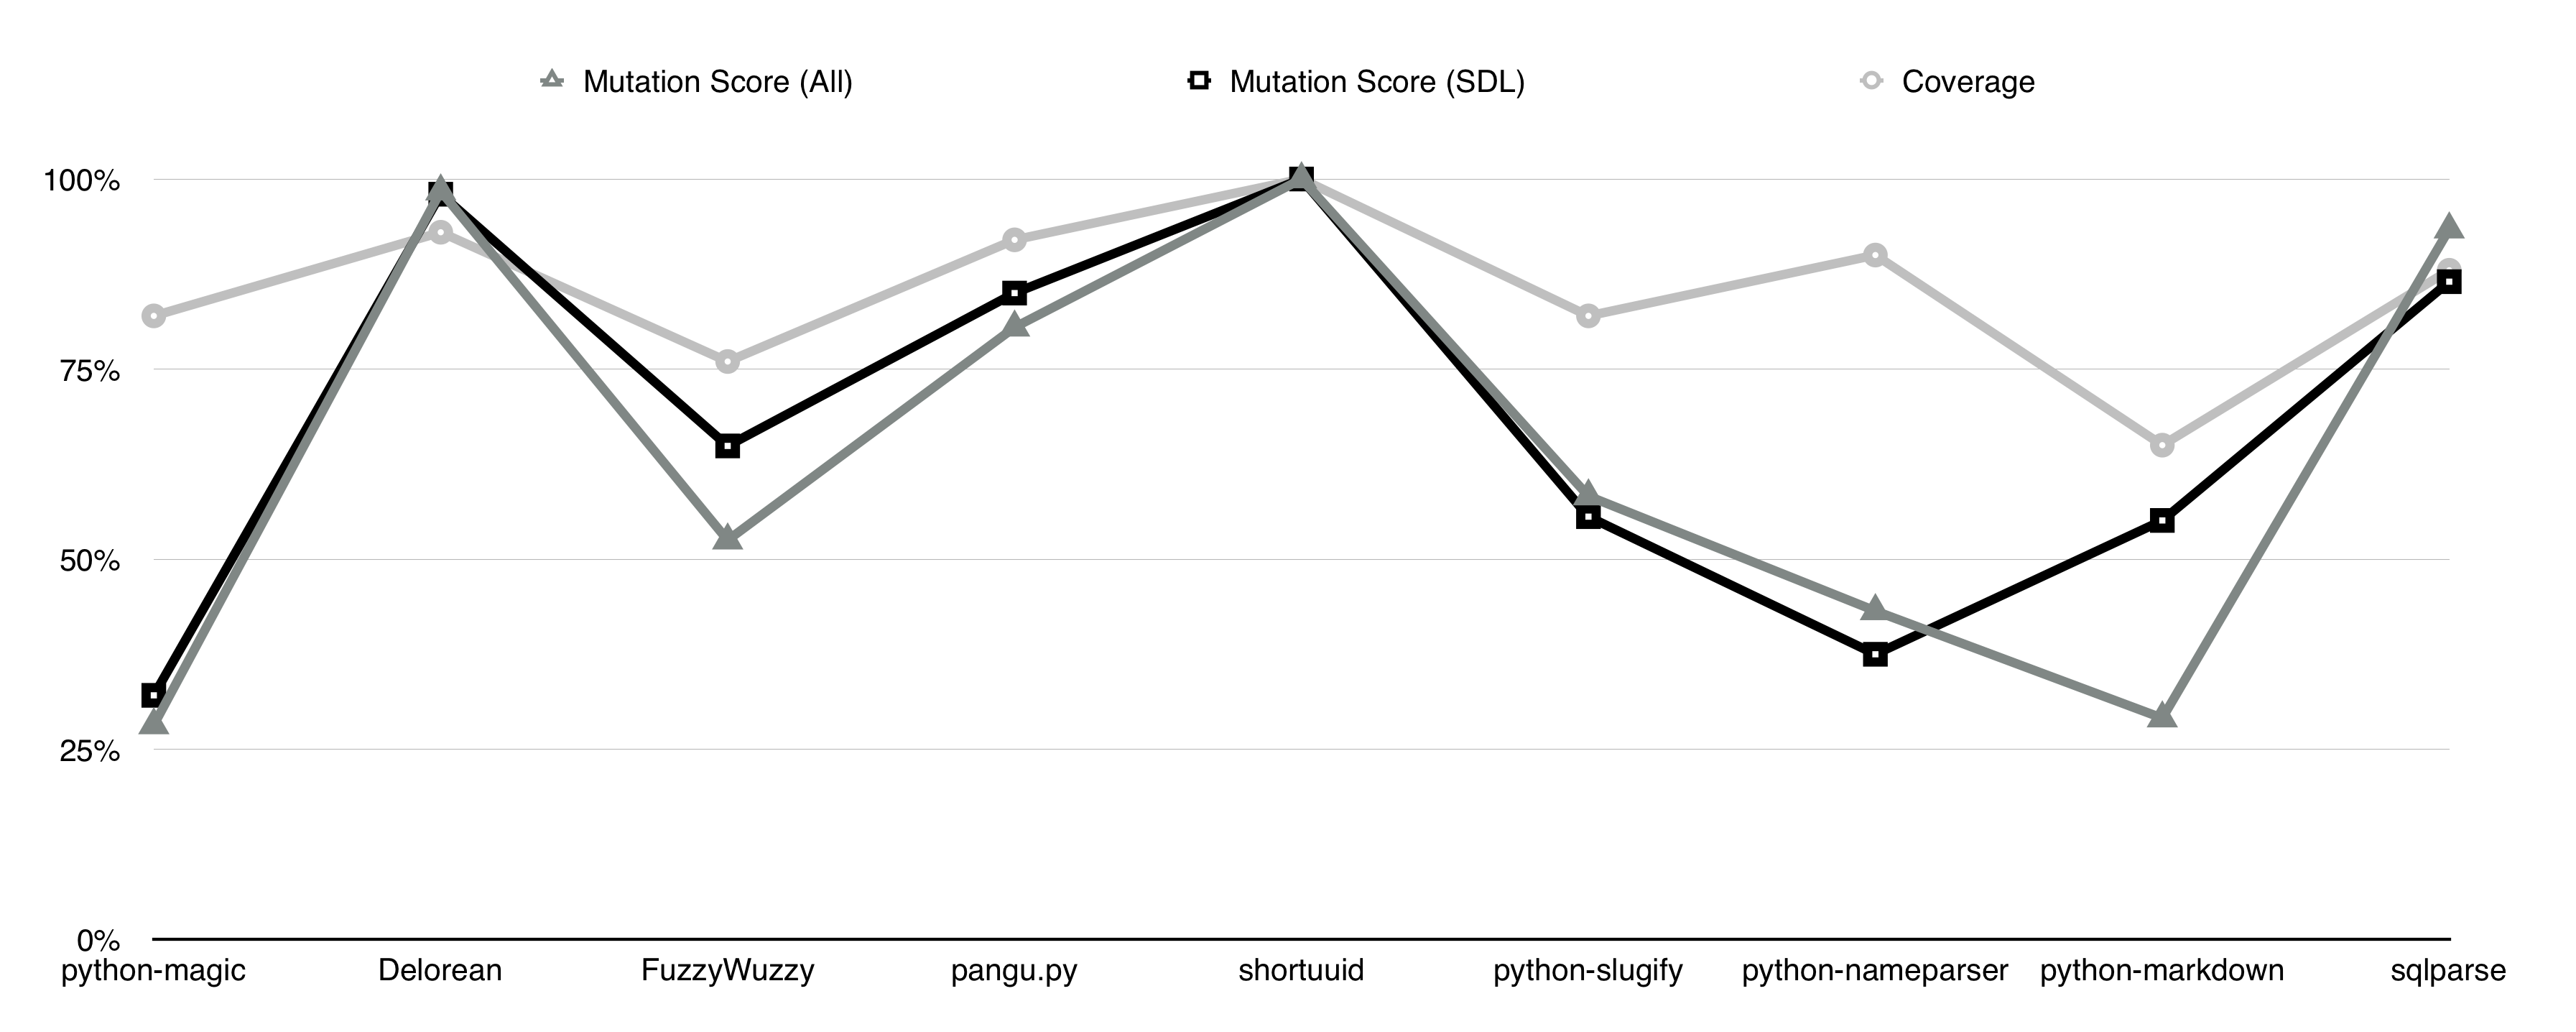
\includegraphics[width=15cm]{score}
\end{center}
\end{figure}

\begin{table}[H]
\begin{center}
\caption{Time usage of mutation testing and coverage}
\label{table:time}
\begin{tabular}{|l|r|r|r|}
\hline
{\bf Project} & {\bf MutPy (All)} & {\bf MutPy (SDL)} & {\bf Coverage} \\
\hline
python-magic      &   57.17s & 39.01s & 0.08s \\
Delorean          &   52.44s & 11.65s & 0.29s \\
FuzzyWuzzy        &   43.98s & 12.34s & 0.33s \\
pangu.py          &    2.63s &  0.68s & 0.20s \\
shortuuid         &   11.57s &  1.38s & 0.28s \\
python-slugify    &    5.54s &  1.22s & 0.09s \\
python-nameparser &  189.72s &  4.15s & 0.74s \\
python-markdown   & 1887.73s & 19.32s & 1.20s \\
sqlparse          &  648.03s & 97.45s & 8.49s \\
\hline
\end{tabular}
\end{center}
\end{table}

\begin{figure}[H]
\begin{center}
\caption{Comparison of time usage between all operators and SDL operator}
\label{fig:time}
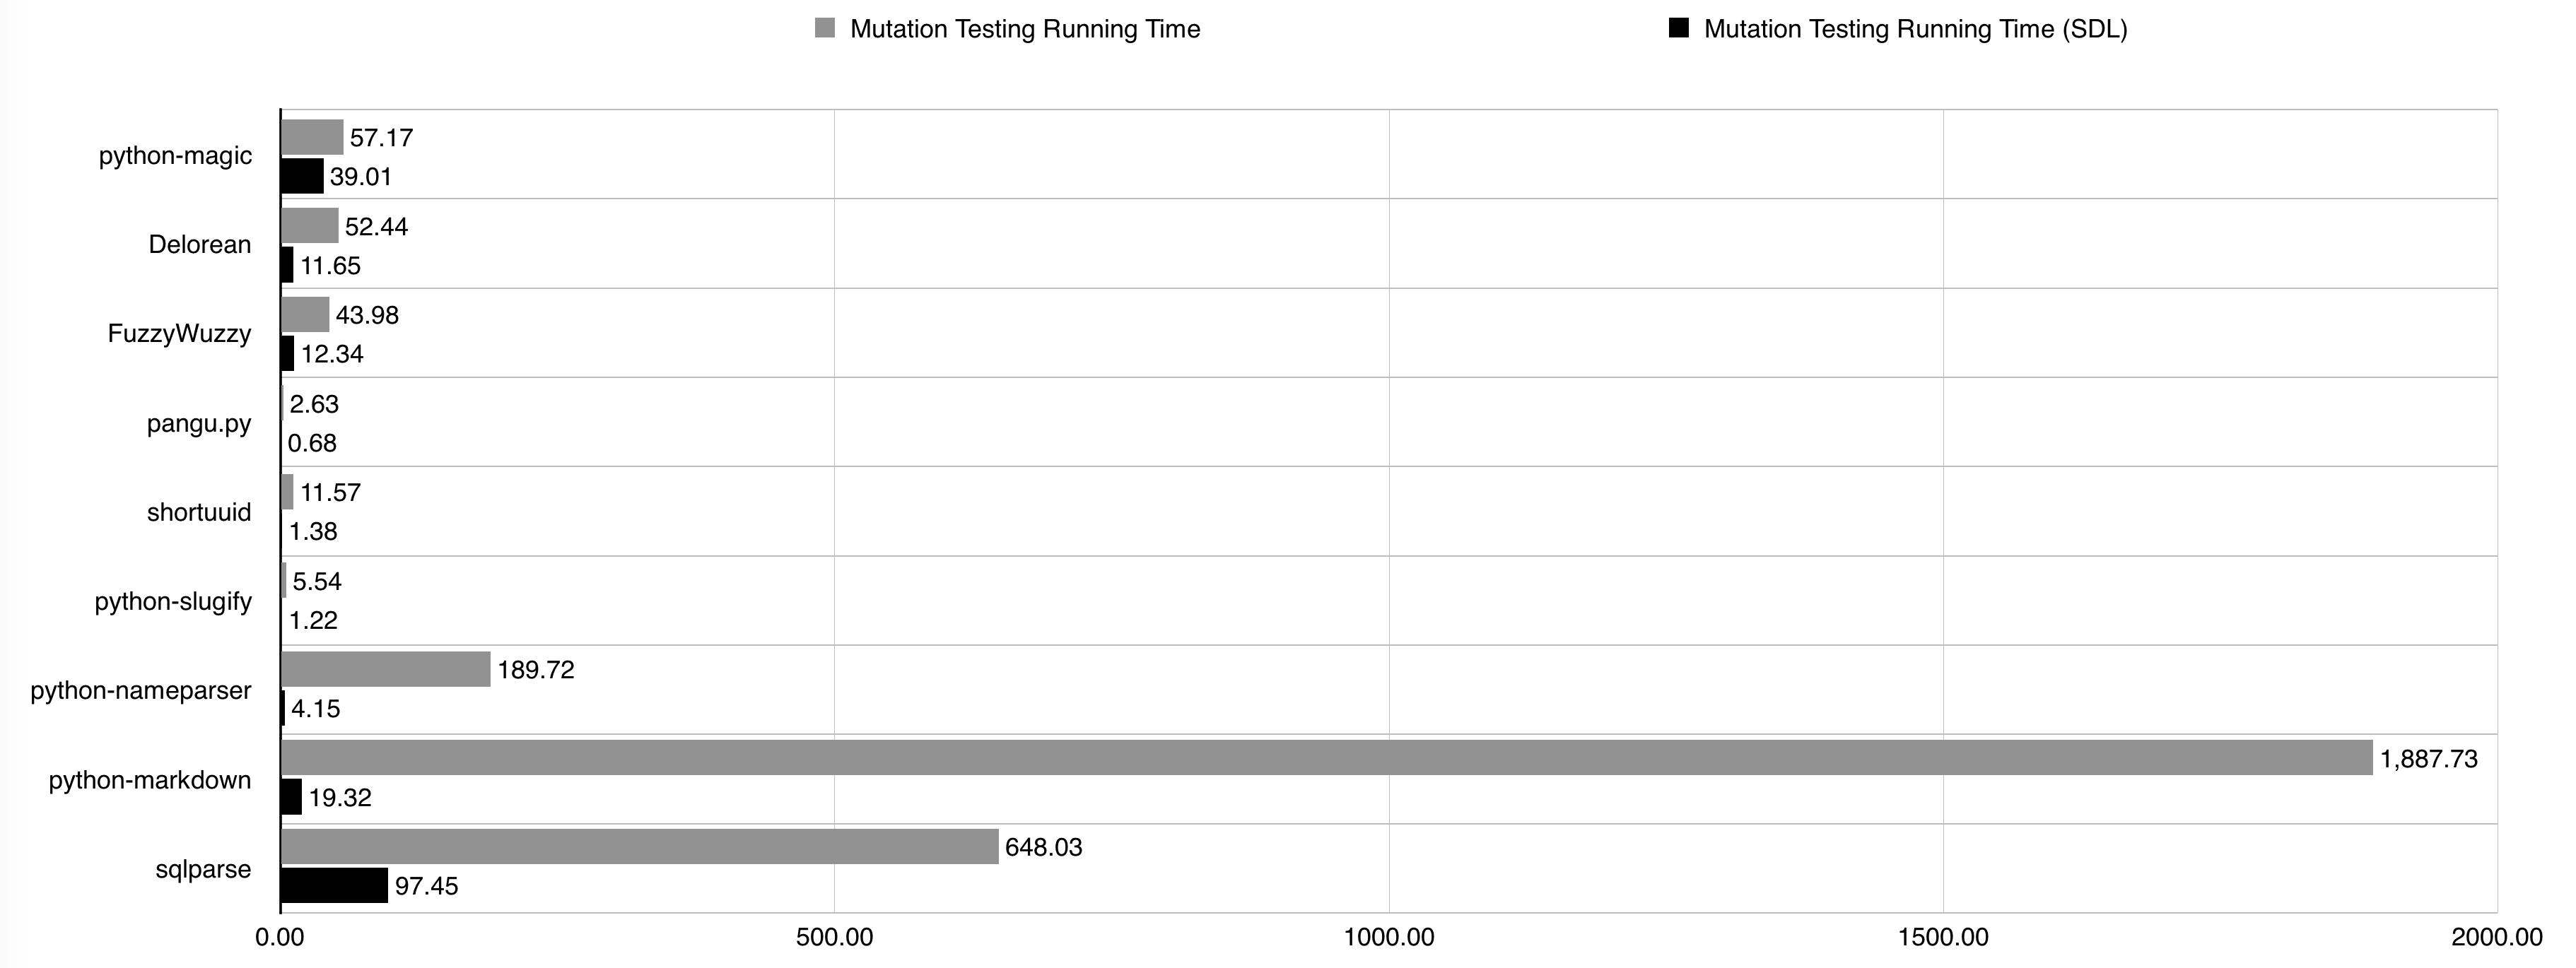
\includegraphics[width=15cm]{time}
\end{center}
\end{figure}

\subsection{Discussion}

As can be seen in Figure \ref{fig:score}, SDL-mutation score is strongly correlated with mutation score using all operators. It also shows the ineffectiveness of traditional test coverage.

In Figure \ref{fig:time}, we can see that SDL-mutation is significantly faster than full mutation testing.  Based on Table \ref{table:time}, SDL-mutation only takes 6.46\% of the time compared to full mutation testing. It is also obvious to see that SDL-mutation is orders of magnitude slower than running traditional unit test coverage. However, we do think SDL-mutation score has some potential to replace traditional coverage. In most of the projects we have evaluated, SDL-mutation testing could be done in 20 seconds. In the biggest project sqlparse, which has 19,434 lines of code, SDL-mutation testing took 97.45 seconds to run. The performance of SDL-mutation testing is acceptable in scenarios like continuous integration.

There are some cases like python-magic where SDL-mutation takes almost the same amount of time compared with full mutation testing. Our analysis showed that the biggest reason is that sometimes MutPy would form an infinite loop in SDL mutant. For each infinite loop, it takes 5 seconds, which is the timeout value in MutPy, to execute. We have proposed a solution in the Future Work section.

\section{Future Work}

Based on our evaluation, we think that there are many potential future work for SDL operator, and mutation testing in general.

\subsection{Extend MutPy Support}

Currently MutPy only loads unit tests based on the Python standard unittest module. However, there are many popular Python projects that do not use the unittest module, including \emph{requests} \cite{requests}, \emph{virtualenv} \cite{virtualenv}, and \emph{Jinja2} \cite{jinja2}. It would be good if MutPy could support different kinds of unit tests in Python projects.

\subsection{Set Timeout Wisely}

A big issue for mutation testing with SDL operator is that after removing a statement, it could form an infinite loop. Currently, MutPy uses a 5s timeout to restrict the running of a test. If a test uses more than the timeout to execute, MutPy would stop the test. However, this approach is not ideal in two ways: First, the infinite loops slow down the execution of the whole test suite. Second, in some applications, e.g. a downloading tool, a passed test may take more than 5s to execute. Stopping such test is not appropriate.

To resolve this issue, we can record the running time for all the tests before running mutation testing. For each test, we set the timeout separately based on its running time. E.g., we can use 10x running time as the timeout.

\subsection{Run Tests Selectively}

Mutation testing is slow because it runs the whole test suite for every mutant. However, there are many cases where a test and a mutant are not relative to each other, so that that test is not possible to kill the mutant. If we can get the coverage information for every test in advance, for each mutant, we can run only the subset of the test suite that covers the mutant, which is significantly smaller than the whole test suite.

\subsection{Investigate the Relevancy Between Survived Mutants and Bugs}

Our evaluation shows that using only SDL operator can get the approximate mutation score. Researches on the relevancy between survived mutants and known bugs would be useful. We would like to see number of bugs per line in code covered by mutation testing, in code covered by SDL-only mutation testing, and in all code.

\subsection{Explore Appropriate Use Cases for Mutation Testing}

Mutation testing is slow because it has to mutate every single line of code multiple times. If we could find some use cases where the lines of code to mutate is small, the mutation testing process would be much faster.

One scenario we can think of is using mutation testing as a pre-commit hook. Before a programmer pushes code, we run mutation testing on the lines they changed. This enforces that the developer who makes the change is also responsible for adding good quality tests for it. Because number of lines is small, the testing could be done in a short amount of time. Scenarios like this are very suitable for mutation testing.

\section{Conclusion}

Untch \cite{untch2009reduced} and Deng \cite{deng2013empirical}'s researches show that the statement deletion operator (SDL) is very effective when performing mutation testing. We extended from their work, evaluated SDL operator on real-world Python projects using MutPy.

Our evaluation shows that in real-world Python projects, SDL-mutation also shows its effectiveness. In our experiments, SDL-mutation score is strongly correlated with full mutation score, while SDL-mutation only take \textbf{6.46\%} of the time in average compared to full mutation testing. We also proposed an idea to reduce the time usage for SDL-mutation even further.

The idea of using one selective operator (SDL) in mutation testing is very interesting. We think that the experiment should be expanded to more and larger Python projects. To support a larger experiment, we would like to see some improvements on test loading to MutPy.

\bibliographystyle{unsrt}
\bibliography{references}

\end{document}
